\documentclass{article}

\usepackage{graphicx}
\usepackage[utf8]{inputenc}
\usepackage{natbib}
\usepackage{float}
\usepackage{natbib}
\usepackage{subcaption}
\usepackage{algorithm}
\usepackage{algorithmic}

\newlength\myindent
\setlength\myindent{2em}
\newcommand\bindent{%
  \begingroup
  \setlength{\itemindent}{\myindent}
  \addtolength{\algorithmicindent}{\myindent}
}
\newcommand\eindent{\endgroup}


\title{Trajectory Modification with Sparse Feedback}
\author{James Staley} 
\begin{document}

\maketitle

\section{Problem Statement}

Agents that can modify how they performs specific tasks based on live user feedback can operate more efficiently, provide better service and will be incorporated more naturally into the lives of regular people. Commercially produced agents will be released with a diverse set of off-the-shelf set of abilities, but standard implementations may not cover every individuals needs. Regular people's lives and homes are filled with innumerable quirks and context specific optimalities. A user must be able to to adjust an agent's behavior to fit their own needs and circumstance. In addition, a user who is able to customize their personal agent's actions may also feel a greater sense of self-actualization and agency over the actions of the robot. Recent HRI research has shown that customizability is critical in delivering independence to the user and creating a positive assistive experience \cite{bhattacharjee_community-centered_2019}. 

We allow for the stylistic customization of a robot arm's movement using a tiled DynaQ learning algorithm that takes simple feedback provided by a user. We attempted to encourage an arm to perform a stylish loop-the-loop motion on its way to the goal.

\section{Background}

Incorporating feedback into reinforcement learning systems is a focus of modern research. There have been several attempts to customize agent trajectories with human feedback. Cui et al. and Argall et al. both corrected a mobile agents trajectory by hand labelling specific past samples as good or bad \cite{cui_active_2018} \cite{argall_learning_2007}. This approach produced good results, but it required a hand-made interface to give criticism and a technical understanding to know which samples should be critiqued. Ideally the feedback interface should be wholly non-technical. A non-technical person can recognize bad behavior in a robot as well as a roboticist, and so better feedback interfaces can benefit all of robotics. 

Other reinforcement learning algorithms incorporate feedback more intuitively. Policy Shaping \cite{griffith_policy_2013} takes binary feedback from a user for state-action pairs and uses it to determine a policy. It then combines that policy with a traditionally (goal based) learned policy at action selection time in order to decide what to do. Policy Shaping works well but relies on difficult to derive parameters about how consistent the coach is and likely they are to provide feedback. Another algorithm, TAMER \cite{knox_reinforcement_2012} accepts feedback to form a selection policy that it then linearly combines with its traditionally learned policy to select an action. In high frequency environments, TAMER credits feedback to multiple samples based on a distribution. TAMER and Policy Shaping have both been used on games and agent behavior, but not to alter robot arm trajectories. We use a TAMER like algorithm, described in the next section, to add sylistic flair ot an arm's trajectory with sparse feedback.

\section{Algorithm}
For the learning representation we implemented Tiled Tabular DynaQ. Q-learning is the simplest version of one-step tabular learning. The agent selects an action $A$ in state $S$ to move to state $S'$. The agent updates the value of its current state-action based on the reward $R$ gained by the transition and the difference between the maximum value of the next state and the value of the current state-action (eqn \ref{eqn:eqn0}. Q-learning follows an $\epsilon-greedy$ policy that selects the best possible action for its state most of the time, and explores $\epsilon$-percent of the time. Over many episodes the agent learns which state-actions have high value by propagating any reward it finds throughout the table.

\begin{equation}\label{eqn:eqn0}
    % \alpha \leftarrow \text{Learning Rate}
    % \gamma \leftarrow \text{Discount Factor}
    Q(S,A) = Q(S,A) + \alpha * [R + \gamma * \max Q(S',a) - Q(S,A)]
\end{equation}

Dyna-Q \cite{sutton_introduction_1998} upgrades Q-learning by planning in the background using a model of the $(s,a,s',r)$ transitions that the agent has experienced. Every time the agent takes an action it updates its model of the environment. The agent simulates $n$ steps using this model for every action it takes in the environment, allowing any discovered reward to propagate around the Q-table much faster than if the agent had to fill out the table by acting. Figure \ref{fig:dyna} shows how we were able to reach asymptomatic performance for the arm achieving its gaol much faster with DynaQ than with just Q-learning.

\begin{figure}[t]
  \centering
    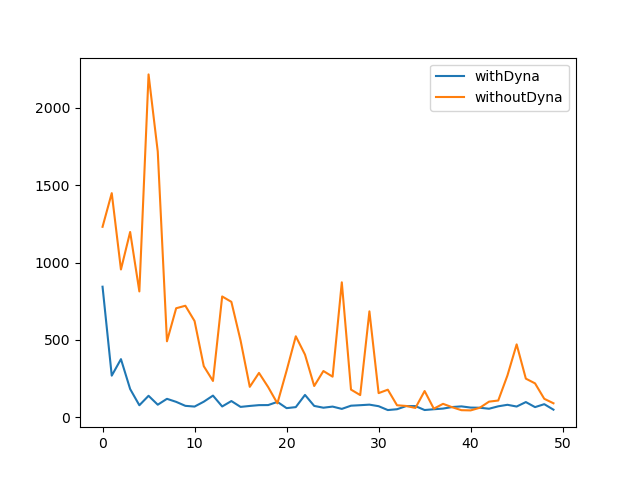
\includegraphics[width=\linewidth]{episodicComparison-5experiments-50episodes.png}
\caption{Asymptomatic performance (steps-per-episode) is reached in fewer episodes (x-axis) with DynaQ.}
\label{fig:dyna}
\end{figure}

We hold two Q tables, $Q$ is the traditional table which is updated from environmental rewards. $\hat{H}$ is a table of identical dimensions, but updated from human feedback. Both tables are updated by DynaQ in order to propagate their rewards faster, they use a separate models. $\hat{H}_{model}$ models the human feedback, and $Q_{model}$ models the environmental reward. 

At greedy action selection time we choose the action with the highest score after adding the weighted feedback values (equation \ref{aselection}).

\begin{equation}\label{aselection}
  a = \max(Q(s,a) + w * \hat{H}(s,a))
\end{equation}

\subsection{Tilings}

Tiling is a way to discretize continuous state spaces. A set of n-dimensional tilings are created that partition the state space. A state will fall into one single partition on each tiling, producing a representation of the state equal in size to the number of tilings. Each of the tilings are offset from one another to prevent patterns in tile activation. Representing continuous states this way lets you discretize the space without the arbitrary breaks that would occur if you implemented a straightforward discretization. The great and generous Richard Sutton has published tiling code in the open source community \cite{sutton_tile_nodate} and we're using an unmodified version for this application. 

Tiling was necessary to build a well functioning learning system for the continuous arm, but it introduced serious resource constraints. The max value of a tiling must be high to prevent tile-value collisions (hash collisions). We were limited to using 3 tilings each with a max value of 2000 for size issues. Both $Q$ and $\hat{H}$ were $2000x2000x2000x5$ dimensional matrices. Since we ran these experiments on a laptop, these stringent resource requirements reduced our ability to expand other dimensions, such as the action space, and limited what we could implement. This was a major failing of our study.

\subsection{Environment}

We found an implemented 2-DOF robot arm training simulator on github \cite{zhou_train-robot-arm--scratch_2019} that used an actor-critic, model-free algorithm based on deterministic policy gradients \cite{lillicrap_continuous_2015}. We removed all the learning code from this project and use the algorithm described above so we could focus on the learning from human feedback.

\begin{figure}[t]
  \centering
  \begin{subfigure}{.225\textwidth}
    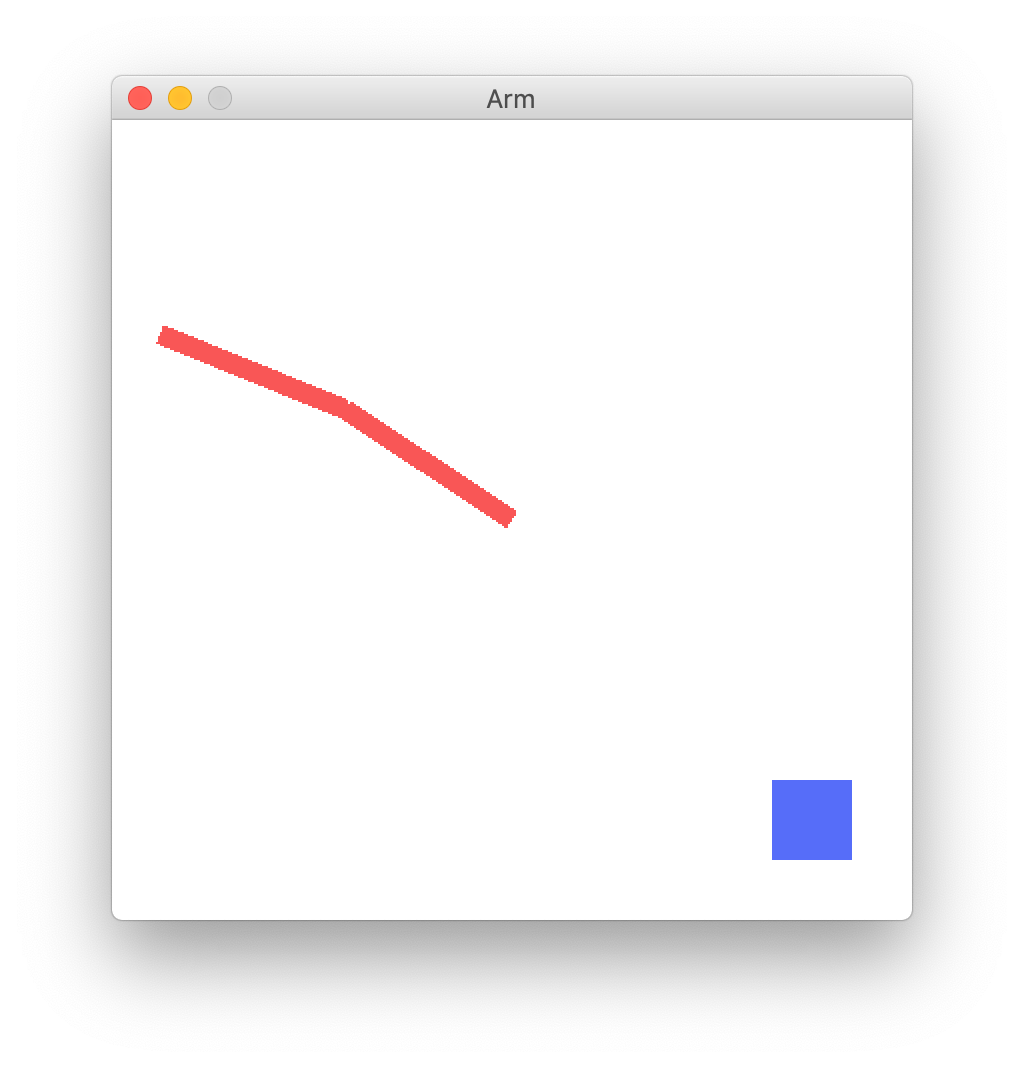
\includegraphics[width=\linewidth]{arm0.png}
  \end{subfigure}
  \begin{subfigure}{.225\textwidth}
    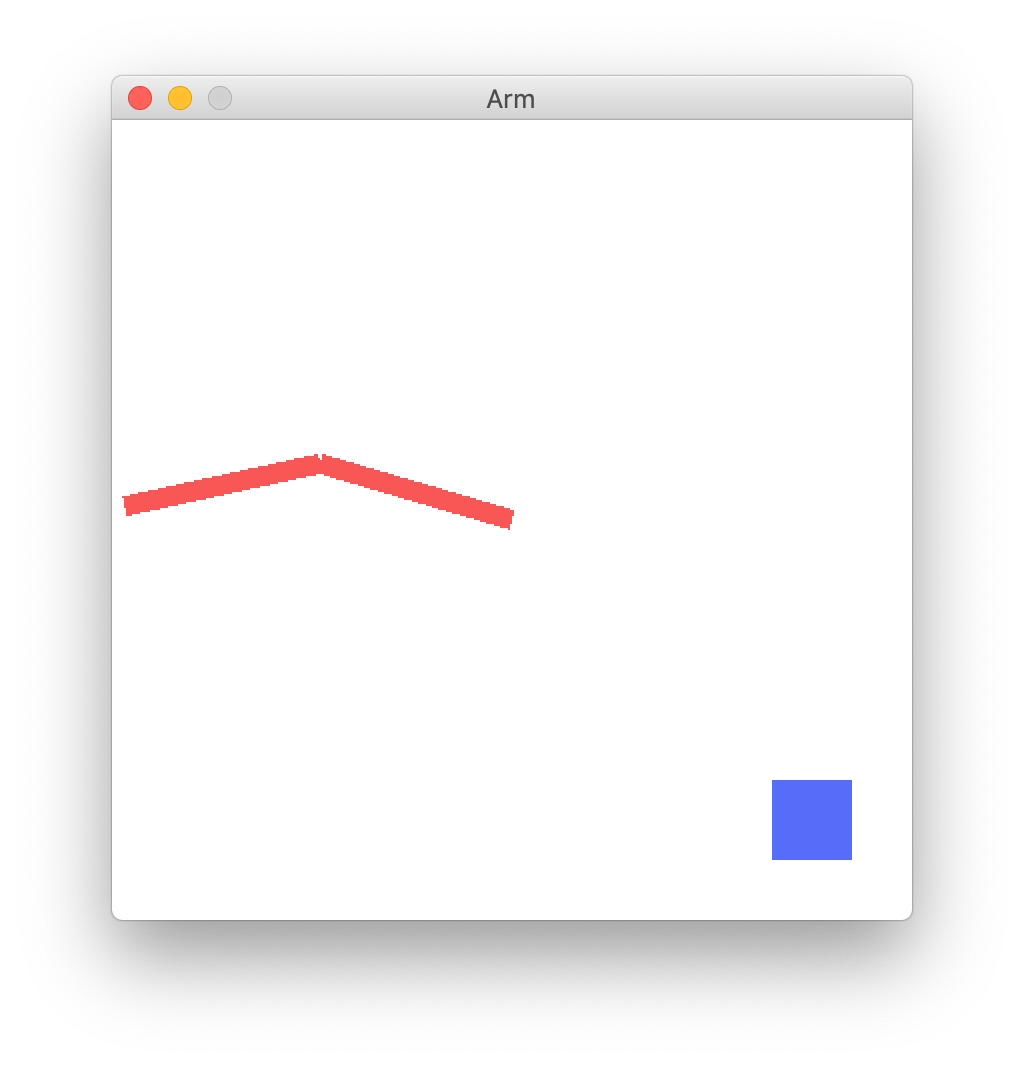
\includegraphics[width=\linewidth]{arm1.png}
  \end{subfigure}
  \begin{subfigure}{.225\textwidth}
    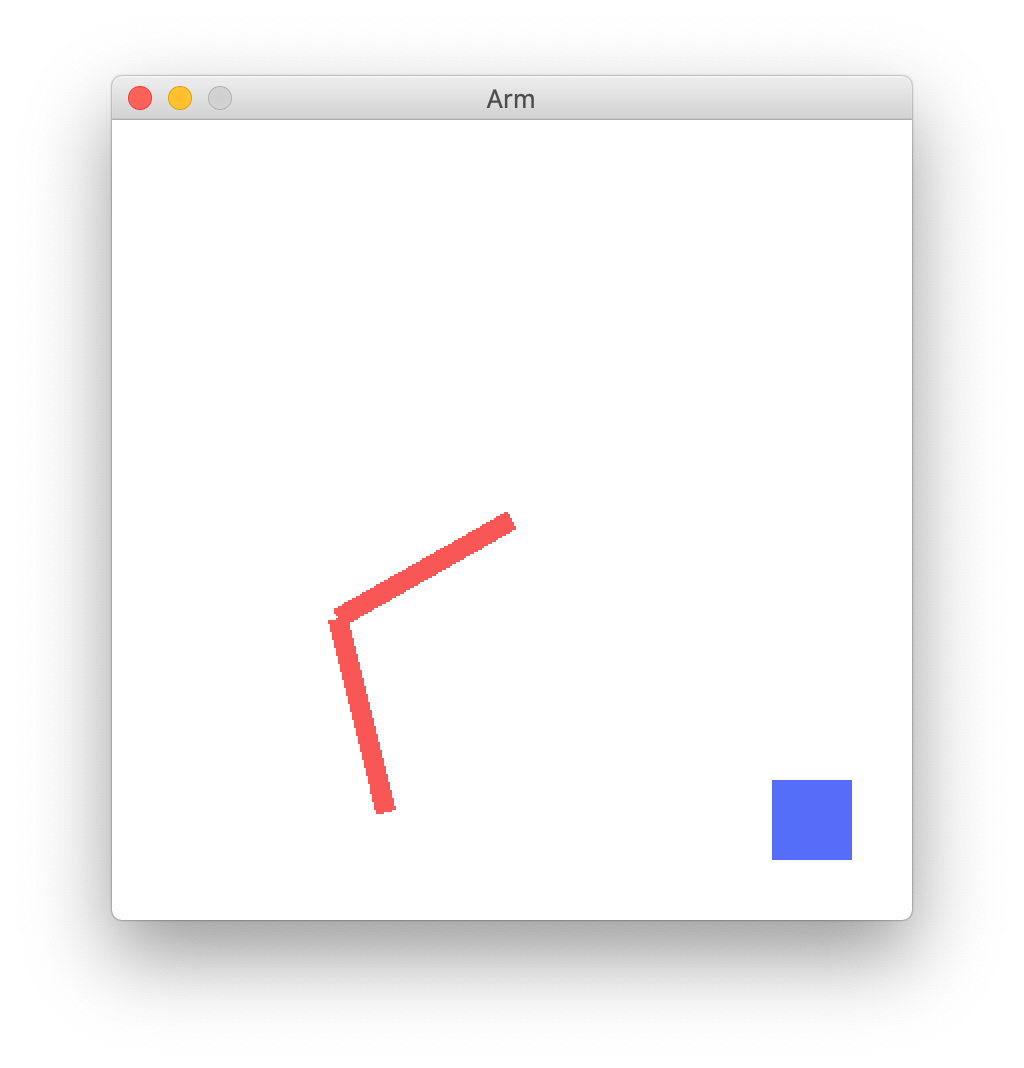
\includegraphics[width=\linewidth]{arm2.png}
  \end{subfigure}
  \begin{subfigure}{.225\textwidth}
    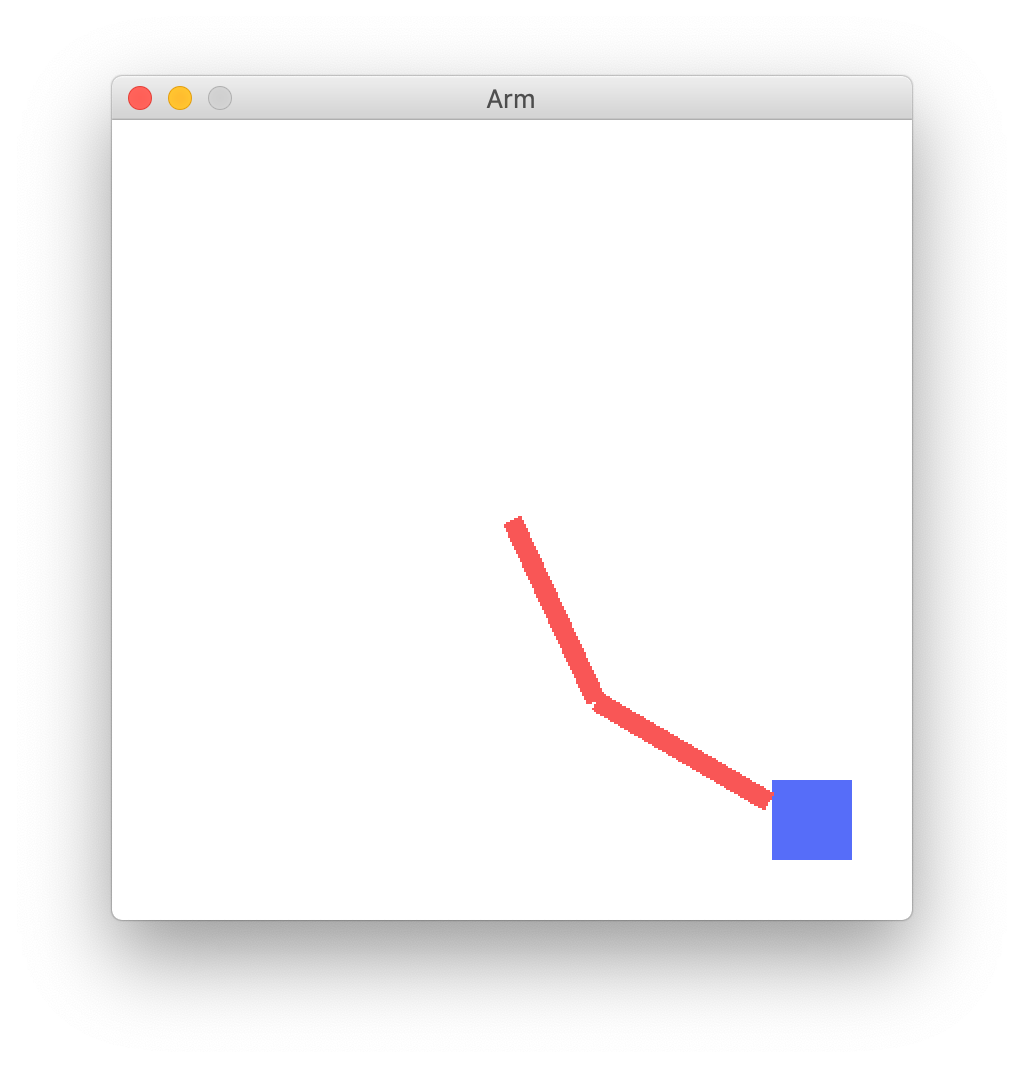
\includegraphics[width=\linewidth]{arm3.png}
  \end{subfigure}
\caption{The 2-DOF trained arm moves towards its goal.}
\label{fig:env-example}
\end{figure}

Fortunately the environment itself could still be used and would save us the time of building our own (figure \ref{fig:env-example}). We modified the environment to work with our learning representation to allow feedback to alter the behavior of the trajectory. 

\subsection{State-Action Representation}

Our agent could take one of four actions. (1) Move the base arm segment clockwise or (2) counter-clockwise by $dtheta$ or (3) move the end-effector clockwise or (4) counter-clockwise by $dtheta$.

The state was the current angular position of each segment of the arm and a brief history of the agent's actions. The last 3 actions were stored in the state to incorporate temporal features into an otherwise markovian model.

\subsection{Subjective Feedback}

We implemented a class, named Subjective, to offer subjective feedback to the agent as it learns. Subjective looks over a windows of history. The history that subjective views is longer than the history held in the agent's state, so the agent has to strategize to keep the subject happy with less information. It follows the simple algorithm shown in Algorithm \ref{alg:subjective}.

\begin{algorithm}
  \caption{Subjective Feedback} \label{alg:subjective}
  \begin{algorithmic}
    \STATE Initialize feedback policy $F(S)$
    \WHILE{True}
      \STATE $(s,a,s') \leftarrow env(a)$
      \STATE $history \leftarrow (s,a,s')$
      \STATE if $random() > 0.95$:
      \bindent
        \STATE $score \leftarrow viewHistory()$
        \STATE $learner.acceptFeedback(score)$
      \eindent
     \ENDWHILE
  \end{algorithmic}
\end{algorithm} 

The Subjective we implemented was trying to encourage loop-the-loops, so it gave a higher score for consistent, non-zero commands to the end-effector of the arm. It gave a negative score for changing the direction of commands to the second arm-segment.

\subsubsection{History}

A history of $(s,a,s')$ was kept. The 100 most recent entries were available for query. Subjective looked through 20 sample windows of the history and gave the highest scoring window to the learner to update $\hat{H}$. 

\subsection{Additional tweaks}

We're doing something a little odd in combining $Q$ and $\hat{H}$. Q is a MDP with a terminal state (the arm reaching the box). Meanwhile, $\hat{H}$ is non-markovian because the best action for a state depends on the agent's history and the loop-the-loop has no terminal state. We get around this with a few modifications of the base algorithm. First, we allow the system to train for 25\% of the total episodes before Subjective says anything. This means that $Q$ forms a consistent policy that prioritizes goal attainment before its behavior is skewed by feedback. Then, once feedback starts, we increase our liklihood of selecting a random action, $\epsilon$, and slowly reduce it back to its baseline. This is to allow for the discovery of policies that maximize the human feedback value $\hat{H}$. These two teaks together create behavior that can perform a loop-the-loop while still achieving the goal. 

TODO: GRAPHS FOR RANDOM RESTART
TODO: PROOF PAPER, then just hand it in

\section{Results}

We found that the agent was able to be trained to do loop-the-loops while still achieving its goal. We were unable to produce graphical examples of this behavior, but the videos found in the presentation linked below show examples of how the agent performs. 

This system was surprisingly sensitive to the parameters that governed learning. If the human feedback was weighed too highly, the agent would happily perform only loop-the-loops and ignore the goal entirely. If the agent did not explore sufficiently, it would never try enough loops to seek them out, and instead only puruse the goal. As you can see in the presented videos, the agent never found a totally smooth balance between its environmental goal (seek the square) and its human-feedack goal (loop-the-loop), but it did find multiple paths that achieved both. The final video in the presentation shows this the best, with the agent directly pursuing the goal via a single loop that completes very near to the goal.  

This experiment demonstrates why combining a markovian goal and a non-markovian goal is a bad idea. The system can learn the desired behavior, but it clearly does not converge to that behavior. A user would have to supervise the agent until it was performing the desired combination of the two goals and then freeze learning, this approach is impractical, requires human oversight, and conflicts with the stated goals of adaptable, user-friendly learning. 

\section{Links}

The project repository can be accessed at https://github.com/dirkmcpherson/reinforcement-learning/tree/master/tufts/final-project

The presentation of this project, including videos, can be found at https://docs.google.com/presentation/d/13K5aZEIK0JH4U0TDkoKMD_SiZyz_IO1OupLfK-9WAIg/edit?usp=sharing

\bibliographystyle{plain}
\bibliography{final_report}
\end{document}

